\documentclass[12pt]{betterjournal}



\graphicspath{ {./images/l2} }

\title{Lab Assignment 2 }

\author{}
\date{}

%New command to display footnote whose markers will always be hidden
\let\svthefootnote\thefootnote
\newcommand\blfootnotetext[1]{%
  \let\thefootnote\relax\footnote{#1}%
  \addtocounter{footnote}{-1}%
  \let\thefootnote\svthefootnote%
}

%Overriding the \footnotetext command to hide the marker if its value is `0`
\let\svfootnotetext\footnotetext
\renewcommand\footnotetext[2][?]{%
  \if\relax#1\relax%
    \ifnum\value{footnote}=0\blfootnotetext{#2}\else\svfootnotetext{#2}\fi%
  \else%
    \if?#1\ifnum\value{footnote}=0\blfootnotetext{#2}\else\svfootnotetext{#2}\fi%
    \else\svfootnotetext[#1]{#2}\fi%
  \fi
}

% Set custom header spanning both columns
\setlength{\headheight}{15.2pt}
\pagestyle{fancy}
\fancyhf{}  % Clear the default header/footer
\fancyhead[R]{ECE/CS 3700}  % Right-side header content
\fancyhead[L]{Lab 2: Simulation and Synthesis}  % Left-side header content

\setlist[itemize]{noitemsep}
\setlist[enumerate]{noitemsep}
\raggedbottom

\begin{document}
\captionsetup{tablewithin=section}
\maketitle
\begin{important}[frametitle={Create a project}]
Before beginning this lab, and in all subsequent labs, create a project following the steps outlined in lab 1. Throughout this lab and the labs that follow, \keyword{top} is used to refer to the top-level module. If you have chosen a different naming convention, you will need to adjust accordingly.
\end{important}

\section{Introduction}

In Lab 1 you explored design techniques and principles through multiplexer circuits. The purpose of this lab is to deepen your understanding of digital logic and Boolean algebra. As undergraduate students in the field of digital design, you will now transition from theoretical concepts to practical implementation using Verilog and FPGAs.

The primary objectives of this lab are to:
\begin{enumerate}
    \item Introduce the crucial concepts of simulation and synthesis in digital circuit design.
    \item Familiarize you with adder circuits, a fundamental building block in digital systems.
    \item Provide hands-on experience in testing digital circuits through both simulation and hardware implementation.
\end{enumerate}



Throughout this lab, you will learn how to:

\begin{itemize}
\item Design and implement basic adder circuits using Verilog
\item Utilize simulation tools to verify the functionality of your designs
\item Synthesize your Verilog code for deployment on an FPGA
\item Test and debug your circuits in actual hardware
\end{itemize}

By the end of this lab, you will have been introduced to the complete digital design workflow, from conceptualization to hardware implementation. This experience will reinforce your understanding of digital logic principles and prepare you for more complex designs in future labs.

\clearpage

\begin{extra}[frametitle={Textbook Reading}]
    Although not strictly necessary to complete this lab, it \textbf{strongly} recommended that you review Chapter 3 of the textbook before moving on. Most of what is covered in this lab is given a thorough treatment in Chapter 3.
\end{extra}
\section{Number systems and Binary review}
\noindent\textbf{Bases:}\hfill\break
Every number system has a base that determines its available digits. Some of the most common systems are:
\begin{itemize}
    \item Base 10 (decimal)
    \begin{itemize}
        \item Uses digits $\{0,1,2,3,4,5,6,7,8,9\}$
    \end{itemize}
    \item Base 2 (binary) 
    \begin{itemize}
        \item Uses digits $\{0,1\}$
    \end{itemize}
    \item Base 16 (hexadecimal)
    \begin{itemize}
        \item $\{0,1,2,3,4,5,6,7,8,9,A,B,C,D,E,F\}$
    \end{itemize}
\end{itemize}

In any base-$n$ system, each digit position $p$ represents $n^p$, where $p$ starts from 0 on the right. The value of a number is the sum of each digit multiplied by its place value.
For example, in base 10, the number 132:
\begin{align*}    
132 &= 1 \cdot 10^2 + 3 \cdot 10^1 + 2 \cdot 10^0
\\&= 100 + 30 + 2
\\&= 132
\end{align*}

The same number in hexadecimal (base 16) would be:
\begin{align*}    
84_{16} &= 8 \cdot 16^1 + 4 \cdot 16^0 \\
&= 128 + 4 \\
&= 132_{10}
\end{align*}

\noindent\textbf{Binary number system}\hfill\break
Binary is a base 2 number system. It uses only 0 and 1 as digits, with each position representing a power of 2. This makes binary particularly useful for computers that operate using electrical signals that can be on (1) or off (0).

For example, the decimal number 5 in binary is 101:
\begin{align*}
101_2 &= 1 \cdot 2^2 + 0 \cdot 2^1 + 1 \cdot 2^0 \\
&= 4 + 0 + 1 \\
&= 5_{10}
\end{align*}

\noindent\textbf{Addition and Carrying}\hfill\break
When adding numbers of any base, we follow these rules:
\begin{enumerate}
    \item Begin at the lowest place
    \item Sum the matching place values
    \item If the sum cannot be expressed as a single digit, carry the excess to the next place.
    \item Repeat until all places have been summed
\end{enumerate}

Example: Adding binary 101 (5) and 1:
\begin{equation*}
\begin{array}{r}
  \phantom{+}101_2\\
  +\phantom{10}1_2\\\hline
  \phantom{+}110_2
\end{array}
\end{equation*}

The rightmost column: $1 + 1 = 10_2$, so we write 0 and carry 1
Middle column: $0 + 1 + \text{(carried 1)} = 10_2$, so write 0 and carry 1
Leftmost column: $1 + \text{(carried 1)} = 10_2$, write both digits

Final result:
\begin{align*}    
110_2 &= 1 \cdot 2^2 + 1 \cdot 2^1 + 0 \cdot 2^0 \\
&= 4 + 2 + 0 \\
&= 6_{10}
\end{align*}

This system of carrying digits works the same way in all bases, but binary is our focus for the remainder of the lab.

\label{sec:review}

\section{An Introduction to adders}

\subsection{Learning Outcomes}
The purpose of this section is to introduce you to digital adders. We will cover their design and operation from first principles. For this lab, our focus will be on unsigned addition. Two's compliment addition will be covered in later labs.

\subsection{Half Adder}
\begin{wrapfigure}{l}{0.3\linewidth}
    \centering
\begin{tikzpicture}[
    auto,
    block/.style={
        rectangle,
        draw=black,
        thick,
        fill=blue!20,
        text width=2cm,
        text centered,
        rounded corners,
        minimum height=10em
    },
    line/.style={draw, thick, -latex', shorten >=2pt}
]

% Half Adder block
\node [block] (adder) {Half Adder};

% Inputs

\draw($(adder.north west)+(0,-1cm)$) -- node[above] {a} ++(-1cm,0);
\draw($(adder.north west)+(0,-3cm)$) -- node[above] {b} ++(-1cm,0);
\draw($(adder.north east)+(0,-1cm)$) -- node[above] {sum} ++(1cm,0);
\draw($(adder.north east)+(0,-3cm)$) -- node[above] {$\text{c}_\text{out}$} ++(1cm,0);

\end{tikzpicture}
    \caption{Half adder block diagram}
    \label{fig:hadder}
\end{wrapfigure}%

The half adder is the simplest adder circuit and the one from which all others are derived. \autoref{fig:hadder} depicts the block diagram of a half adder. It has 2 inputs
\begin{enumerate}
    \item \textbf{a:} The left operand
    \item \textbf{b:} The right operand
\end{enumerate}
\clearpage
And 2 outputs
\begin{enumerate}
    \item \textbf{sum:} The result of $\textbf{a} + \textbf{b}$
    \item $\textbf{c}_\textbf{out}$: The carry-out bit
\end{enumerate}%
{\setlength{\linewidth}{\textwidth}
\noindent
This circuit is considered a half adder because it has no input for a carry-in bit. Without a carry-in bit, sums larger than 2 bits are not computable. To get around this limitation, 2 half adders can be connected in series to create a full adder. The truth table for a half adder is given in \autoref{tab:half_adder}.}

% Requires: \usepackage{amssymb}
\begin{table}[htpb!]
    \centering
    \begin{tabular}{cc | cc}
        \toprule
        $A$ & $B$ & Sum & $C_{\text{out}}$ \\
        \midrule
        0 & 0 & 0 & 0 \\
        0 & 1 & 1 & 0 \\
        1 & 0 & 1 & 0 \\
        1 & 1 & 0 & 1 \\
        \bottomrule
    \end{tabular}
    \caption{Truth table for a half adder}
    \label{tab:half_adder}
\end{table}

% Full Adder Section
\subsection{Full Adder}
\begin{wrapfigure}{r}{0.3\linewidth}
    \centering
\begin{tikzpicture}[
    auto,
    block/.style={
        rectangle,
        draw=black,
        thick,
        fill=blue!20,
        text width=2cm,
        text centered,
        rounded corners,
        minimum height=10em
    },
    line/.style={draw, thick, -latex', shorten >=2pt}
]

% Full Adder block
\node [block] (adder) {Full Adder};

% Inputs

\draw($(adder.north west)+(0,-1cm)$) -- node[above] {a} ++(-1cm,0);
\draw($(adder.north west)+(0,-2cm)$) -- node[above] {b} ++(-1cm,0);
\draw($(adder.north west)+(0,-3cm)$) -- node[above] {$\text{c}_{\text{in}}$} ++(-1cm,0);
\draw($(adder.north east)+(0,-1cm)$) -- node[above] {sum} ++(1cm,0);
\draw($(adder.north east)+(0,-3cm)$) -- node[above] {$\text{c}_\text{out}$} ++(1cm,0);

\end{tikzpicture}
    \caption{Full adder block diagram}
    \label{fig:adder}
\end{wrapfigure}

\autoref{fig:adder} depicts a full adder. It takes 3 inputs:

\begin{itemize}
    \item \textbf{a}: The left operand
    \item \textbf{b}: The right operand
    \item $\textbf{c}_\textbf{in}$: The carry in bit from a previous addition if applicable, otherwise 0.
\end{itemize}

And has two outputs:

\begin{itemize}
    \item \textbf{sum}: The sum a + b + $c_\text{in}$
    \item $\textbf{c}_\textbf{out}$: The carry-out bit or 0 if no carry is required.
\end{itemize}

A full adder is created by combining two half adders in series as previously mentioned. \autoref{fig:fadder} is taken from chapter 3 in the textbook and depicts the decomposition of a full adder. \autoref{tab:full_adder_tt} provides the truth table for a single-bit full adder.
\begin{figure}
    \centering
    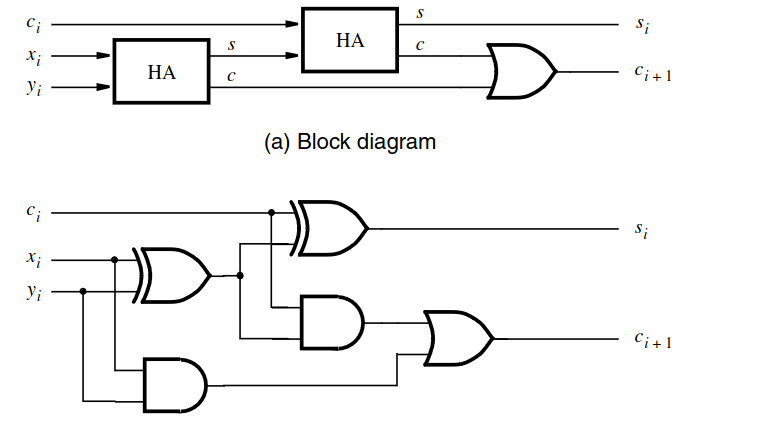
\includegraphics[width=1\linewidth]{fulladderdiagram.png}
    \caption{A decomposed implementation of the full-adder circuit. $c$ is the textbook notation for what the lab refers to as $\text{c}_\text{out}$. $s$ is the textbook notation for sum and $c_i$ is the carry in bit from a previous stage.}
    \label{fig:fadder}
\end{figure}


\begin{table}[H]
    \centering
    \begin{tabular}{ccc|cc}
        \toprule
        A & B & Cin & Sum & Cout \\
        \midrule
        0 & 0 & 0 & 0 & 0 \\
        0 & 0 & 1 & 1 & 0 \\
        0 & 1 & 0 & 1 & 0 \\
        0 & 1 & 1 & 0 & 1 \\
        1 & 0 & 0 & 1 & 0 \\
        1 & 0 & 1 & 0 & 1 \\
        1 & 1 & 0 & 0 & 1 \\
        1 & 1 & 1 & 1 & 1 \\
        \bottomrule
    \end{tabular}
    \caption{Truth table for a 1-bit full adder.}
    \label{tab:full_adder_tt}
\end{table}
\clearpage
\begin{question}[Full adder design]
\begin{enumerate}
    \item  Create a half adder module that receives 2 inputs: $\mathbf{a}$ and $\mathbf{b}$ and provides 2 outputs: \textbf{sum} and $\textbf{c}_\textbf{out}$. Design the logic in either structural or gate-level modeling styles.
    \item Create a full adder module that receives 3 inputs: $\mathbf{a},\mathbf{b}$, and $\textbf{c}_\textbf{in}$ and provides 2 outputs:\hspace{1em}\textbf{sum} and $\textbf{c}_\textbf{out}$. Design the logic using two instances of the half adder module you designed in 1.
\end{enumerate}
\end{question}
\noindent
\textbf{Recall from lab 1:}
\begin{lstlisting}[language=Verilog]
module Mux41Structural (
    input wire ...,
    output wire ..., 
);
    someModule MyModule(.a(...), .b(...), ...);
endmodule
\end{lstlisting}
\section{Your First Test Bench}
Simulation is a crucial first step before implementing any digital design in hardware. Here's why:
\hfill\break
\hfill\break
\noindent\textbf{Risk Reduction:}
\noindent
\begin{itemize}
    \item Simulations provide a safe and cost-effective way of verifying design logic.
    \item Hardware bugs can be expensive and time-consuming to fix.
    \item Design flaws are much easier to correct in simulation than in physical hardware.
\end{itemize}
\hfill\break
\hfill\break
\noindent\textbf{The Simulation-Hardware Relationship:}
\noindent
\begin{itemize}
    \item A successful simulation suggests your logic is sound, but doesn't guarantee hardware success.
    \item However, if your design fails in simulation, it will definitely fail in hardware.
    \item Think of simulation as a necessary but not sufficient condition for hardware success.
\end{itemize}
\hfill\break
\hfill\break
\noindent
\textbf{Best Practice Guidelines:}
\noindent
\begin{itemize}
    \item Always simulate your design thoroughly before moving to hardware implementation.
    \item Test multiple input combinations and edge cases during simulation.
    \item Document and fix all simulation issues before proceeding to hardware.
\end{itemize}
\hfill\break
\hfill\break
\textbf{Remember:} While passing simulation is no guarantee of hardware success, failing simulation is a guarantee of hardware failure.

\subsection{Test Bench Template}
Below is a complete test bench for the half adder design. This test bench can be readily adapted to any unit. We will go through each section and provide a thorough explanation.

\begin{lstlisting}[language=verilog]
`timescale 1ns/100ps    // 1 nanosecond steps, 100 picosecond precision

module HalfAdder_tb();

// 1. Define simulation timestep for readability
`define STEP 10    // Each test case will take 10 time units

// 2. Declare signals
reg a, b;           
wire sum, carry;    

// 3. Instantiate the half adder
HalfAdder uut(
    .a(a),
    .b(b),
    .sum(sum),
    .cout(carry)
);

// 4. Variables for loop and checking
reg [1:0] test_vector;
reg expected_sum, expected_carry;
integer i;
integer errors = 0;

// 5. Initial block with for loop
initial begin
    // Print header
    $display("Time(ns)\ta\tb\tsum\tcarry\tExpected\tStatus");
    $display("--------\t-\t-\t---\t-----\t--------\t------");
    
    // Test all combinations using a for loop
    for (i = 0; i < 4; i = i + 1) begin
        // Convert loop index to test inputs
        test_vector = i[1:0];
        a = test_vector[1];
        b = test_vector[0];
        
        // Calculate expected results
        expected_sum = a ^ b;
        expected_carry = a & b;
        
        // Wait for circuit to settle
        #(`STEP);
        
        // Check and display results
        if ((sum === expected_sum) && (carry === expected_carry))
            $display("%0d\t%b\t%b\t%b\t%b\t%b%b\t\tPASS", 
                    $time, a, b, sum, carry, expected_sum, expected_carry);
        else begin
            $display("%0d\t%b\t%b\t%b\t%b\t%b%b\t\tFAIL", 
                    $time, a, b, sum, carry, expected_sum, expected_carry);
            errors = errors + 1;
        end
    end
    
    // Display final test results
    $display("\nSimulation completed with %0d errors", errors);
    $finish;
end

endmodule
\end{lstlisting}

\begin{enumerate}
    \item timescale and module
    \begin{itemize}
        \item \keyword{timescale:} Every test bench begins with defining a \keyword{timescale}. The simulator cannot run at the speeds required for accurate simulation because it is software and the design is intended for hardware. To simulate these speeds the simulator uses an internal clock. The \keyword{timescale} macro defines how many seconds a single clock tick represents and how precise the timing should be.
        \item \keyword{module:} Everything in Verilog is a \keyword{module} and a test bench is no exception. The convention is to name the module using the pattern \keyword{ModuleUnderTestName\_tb}.
    \end{itemize}
    \item Definitions
    \begin{itemize}
        \item define constants for values you expect to use a lot. STEP in this example will be used as a delay value. Between 10 - 20 is typical.
    \end{itemize}
    \item  Declare Signals
    \begin{itemize}
        \item Declare the signals that will drive the circuit and receive the output. Inputs will always be \keyword{reg} and the outputs will always be \keyword{wire}. The reason for this will be clear when we discuss sequential circuit design in the next lab. For now, it suffices to understand that values that will be changed inside the testbench will always be \keyword{reg}s. Values that are expected to be changed by another module will always be \keyword{wire}s.
    \end{itemize}
    \item Instantiation
    \begin{itemize}
        \item Create an instance of the module to test. Convention is to name the instance \keyword{uut} short for unit under test.
    \end{itemize}
    \item Variables
    \begin{itemize}
        \item Set up any variables that are not constants and are not used to carry or send signals.
    \end{itemize}
    \item {Initial Block}
    \begin{itemize}
        \item Anything inside the \keyword{initial} block runs after variable declarations and instantiations, but before any other block. Because we are using purely combinational logic, the full test goes in here. This will change in the future and we will discuss the changes at that time.
    \end{itemize}
    \item {Test Logic}
    \begin{itemize}
        \item \keyword{\$display:} Print a message to the simulator console
        \item \keyword{for:} Behaves like a typical for loop. Not synthesizable, \textbf{Can only be used in simulation}.
        \item \keyword{begin/end:} Defines a block. Used when a keyword expects a block and doesn't have its own end keyword. IE \texttt{for (...) begin ... end} but not \texttt{module begin ... end}.
        \item \keyword{\# (delay):} Add delay to give the circuit time to propagate and settle. Parentheses are only required when referencing a variable or constant.
        \item \textbf{if/else:} Basic \textbf{if/else} block. Behaves as expected; \textbf{begin/end} keywords required for multiline blocks.
    \end{itemize}
    \item \textbf{\$finish:} End the simulation
\end{enumerate}

Save this file in your tests directory as \keyword{HalfAdder\_tb.v}. Open Questa and create a new project. Add Your \keyword{HalfAdder.v} file and your testbench.

\hfill\break
\begin{question}[Successful Simulation]
    Run your test bench in the Questa software. Verify a successful output by examining the output terminal. Take a screenshot of the output and include it in your lab report.
\end{question}
\section{Ripple Carry Adder}
Now that our full adder design has been simulated successfully, we are ready to design our first complex adder. This design works the same way as the arithmetic algorithm you are familiar with and which was reviewed in Section \ref{sec:review}. A block diagram for the ripple carry adder is given in \autoref{fig:ripplecarry}. The output of the ripple carry is the concatenation of $s_0\cdots s_n$ as a single vector. Recall that concatenation of bits is possible in Verilog like so:
\begin{lstlisting}[language=verilog]
    // assume s0, s1, and s2 are already defined
    wire sum[2:0];
    assign sum = {s2, s1, s0};
\end{lstlisting}
\begin{figure}
\centering
\begin{tikzpicture}[
    auto,
    block/.style={
        rectangle,
        draw=black,
        thick,
        fill=blue!20,
        text width=2cm,
        text centered,
        rounded corners,
        minimum height=2cm
    },
    line/.style={draw, thick, -latex', shorten >=2pt}
]

% Full Adder blocks - positioned horizontally
\node [block] (adder0) {Full Adder};
\node [block, right=2cm of adder0] (adder1) {Full Adder};
% \node [block, right=2cm of adder1] (adder2) {Full Adder};

% Inputs for first adder
\draw($(adder0.north west)+(.5cm, 0)$) |- node[above] {$a_0$} ++(0,1cm);
\draw($(adder0.north east)+(-.5cm,0)$) |- node[above] {$b_0$} ++(0,1cm);
\draw($(adder0.north west)+(0,-1cm)$) -- node[above] {$\text{c}_{\text{in}}$} ++(-1cm,0);
\draw($(adder0.south)$) |- node[below] {$s_0$} ++(0,-1cm);

% Inputs for second adder
\draw($(adder1.north west)+(.5cm, 0)$) |- node[above] {$a_1$} ++(0,1cm);
\draw($(adder1.north east)+(-.5cm,0)$) |- node[above] {$b_1$} ++(0,1cm);
\draw($(adder1.south)$) |- node[below] {$s_1$} ++(0,-1cm);

% % Inputs for third adder
% \draw($(adder2.north west)+(.5cm, 0)$) |- node[above] {$a_2$} ++(0,1cm);
% \draw($(adder2.north east)+(-.5cm,0)$) |- node[above] {$b_2$} ++(0,1cm);
% \draw($(adder2.south)$) |- node[below] {$s_2$} ++(0,-1cm);
% \draw($(adder2.north east)+(0,-1cm)$) -- node[above] {$\text{c}_{\text{out}}$} ++(1cm,0);

% Connect carry bits between adders
\draw[line] ($(adder0.north east)+(0,-1cm)$) -- node[above] {$\text{c}_1$} ($(adder1.north west)+(0,-1cm)$);
\draw[line] ($(adder1.north east)+(0,-1cm)$) -- node[above] {$\text{c}_2$} ($(adder1.north east)+(2cm,-1cm)$);

\end{tikzpicture}
\caption{2-Bit Ripple Carry Adder Block Diagram}
\label{fig:ripplecarry}
\end{figure}
\hfill\break
\begin{question}[4-bit Ripple Carry]
    Design a 4-bit ripple carry adder using the full adder modules you designed and tested previously. Write a test bench following the pattern shown previously. Take a screenshot of the successful output and include it in your report.
\end{question}
\section{Timing and Space}
Although the ripple carry adder is simple and intuitive, the cascading nature of its design renders it inefficient for large sums. The sum and carry values from each stage are not computed instantaneously. Some small amount of time, call it $\Delta{t}$, is required to perform the calculation. Thus the total $\Delta{t}$ for an n-bit adder = $n\Delta{t}$. In addition to the time requirements, there are a finite number of logic elements available on a physical device. The logic elements also scale with $n$.

To see this, we will setup some timing parameters so that Quartus can provide us with accurate timing information.

\section{Synthesis}
To use our timing analysis, we need to first synthesize our design. Quartus needs to be aware of the hardware we are using in order for it to provide accurate timing information. To do this, we must first create a top-level module. In \keyword{top.v} create a module named \textbf{top} just as we did in lab 1. It will receive as inputs 2 4-bit numbers $\mathbf{a}$ and $\mathbf{b}$ It will output a 4-bit number \textbf{sum} and a single \textbf{cout} bit. The block diagram is provided in \autoref{fig:top}

\begin{figure}
    \centering
    \begin{tikzpicture}[
    auto,
    block/.style={
        rectangle,
        draw=black,
        thick,
        fill=blue!20,
        text width=2cm,
        text centered,
        rounded corners,
        minimum height=8em
    },
    line/.style={draw, thick, -latex', shorten >=2pt}
]

% Full Adder block
\node [block] (adder) {top};

% Inputs

\draw($(adder.north west)+(0,-1cm)$) -- node[above] {[4:0]a} ++(-2cm,0);
\draw($(adder.north west)+(0,-2cm)$) -- node[above] {[4:0]b} ++(-2cm,0);
\draw($(adder.north east)+(0,-1cm)$) -- node[above] {[4:0]sum} ++(2cm,0);
\draw($(adder.north east)+(0,-2cm)$) -- node[above] {$\text{c}_\text{out}$} ++(2cm,0);

\end{tikzpicture}
    \caption{Top level module block diagram}
    \label{fig:top}
\end{figure}

\subsection{Pin layout}
Any input or output declared in the top-level module will be interpreted as coming from an external source. The DE-10 Lite FPGA has a variety of inputs and outputs. To assign our top-level ports to these I/Os, we make use of the pin planner.

Before we can access the pin planner, we need to compile the design. Go to\directions{Processing, Start Compilation}. This may take several minutes to complete.

Once the compilation is complete you can access the pin planner through \directions{Assignments, Pin Planner}. This will open a new window that looks something like \autoref{fig:pinplanner}. Your window will not be filled as shown in the image. We will address that now. \hfill\break
\begin{figure}
    \centering
    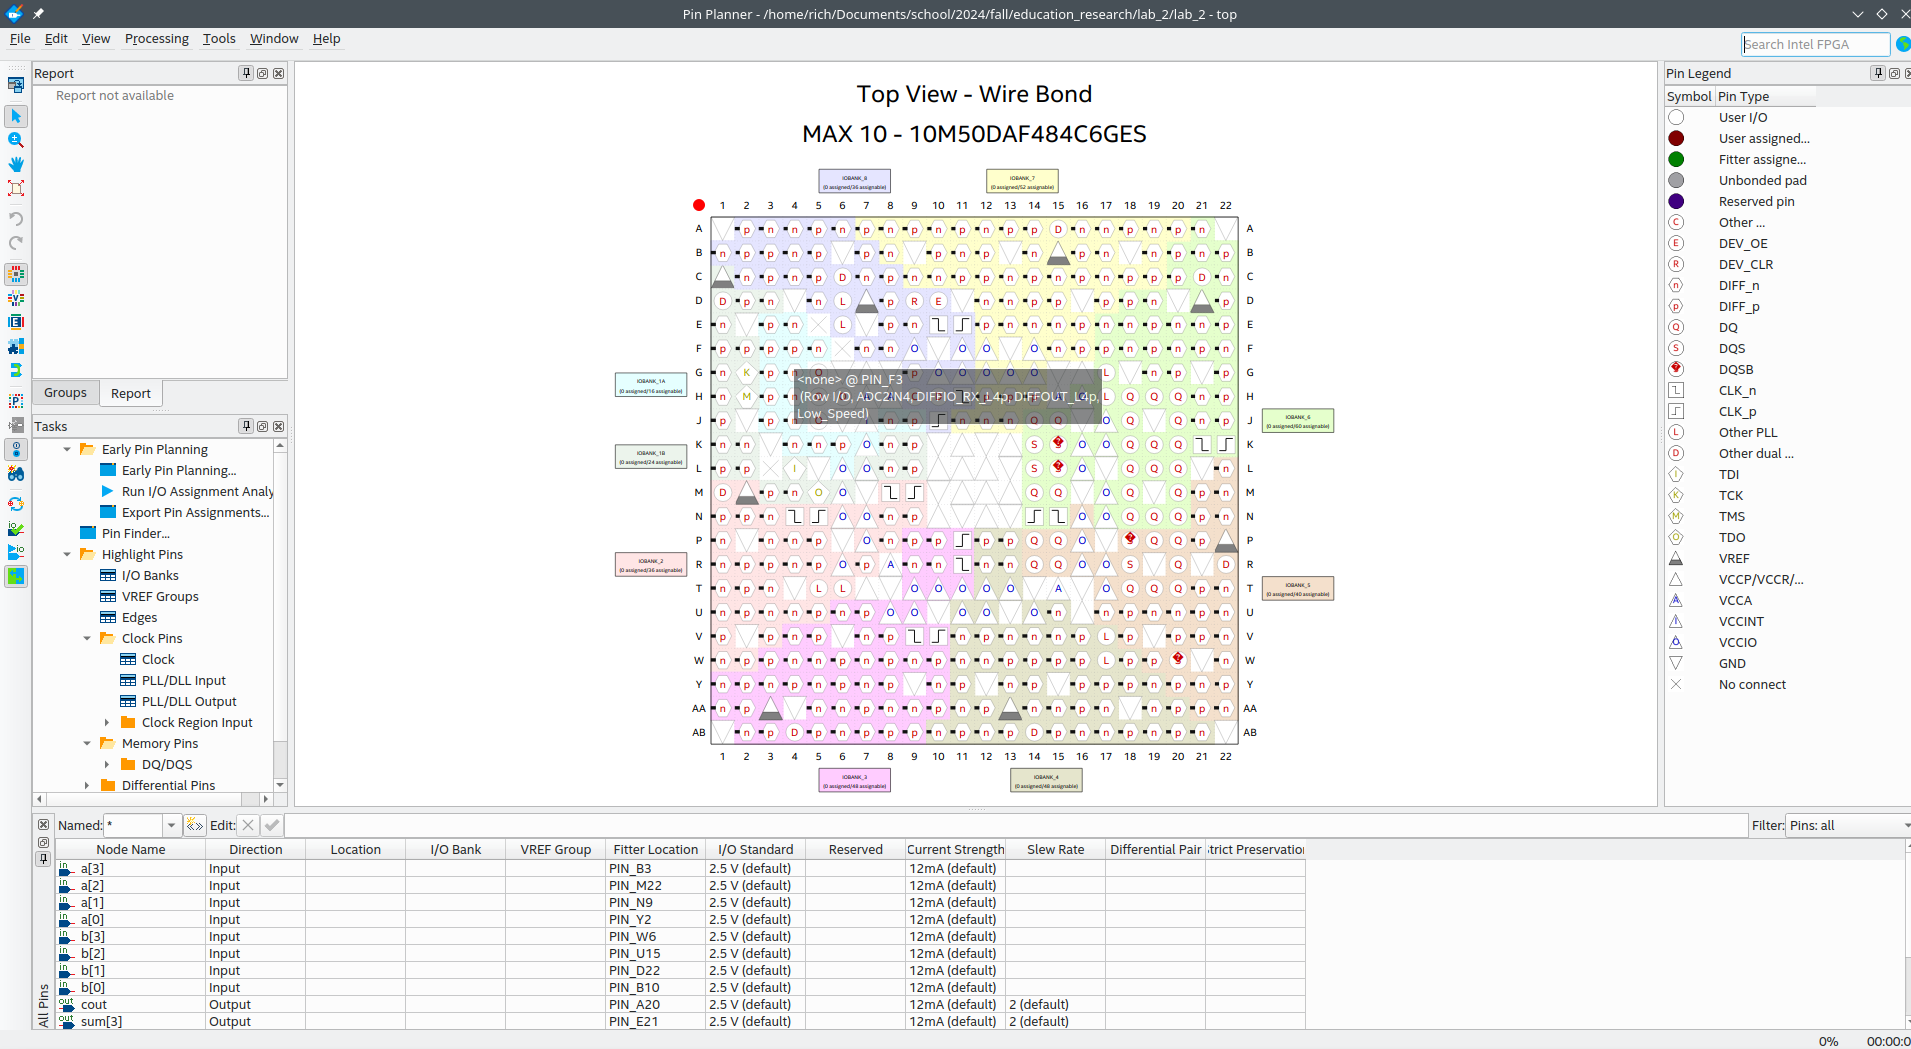
\includegraphics[width=\linewidth]{pinplanner.png}
    \caption{Pin Planner Interface}
    \label{fig:pinplanner}
\end{figure}
\begin{extra}[frametitle={Board Selection}]
    In the pin planner interface you will see above a large grid, the words\hfill\break \textbf{MAX 10 - 10M50DAF484C6GES}. This is the model number of the FPGA you are assigning pins to. If you don't see this name exactly, you have the wrong board selected. In this case, close the pin planner and in the main Quartus window go to:\hfill\break \directions{Assignments, Device}, select the correct device, and recompile. Then open the pin planner and make sure the correct device is now displayed at the top.
\end{extra}

At the bottom of the interface is a table of inputs and outputs defined in your top-level module. If this list is empty, make sure that the inputs and outputs are correctly declared in your \textbf\texttt{top.v} file and that you have successfully compiled your design. \autoref{fig:pinlist} show what a populated list will look like. In your list, the location column will be empty.

\begin{figure}
    \centering
    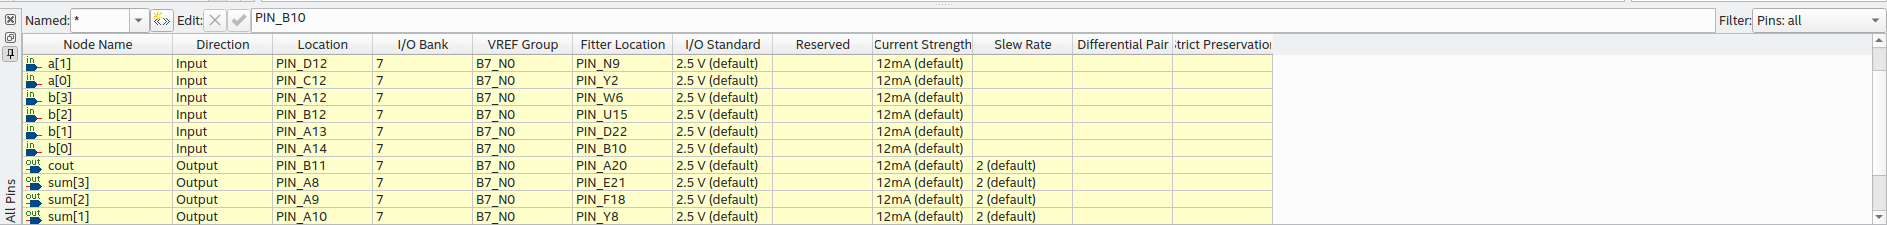
\includegraphics[width=\linewidth]{pinplannerpins.png}
    \caption{List of pin assignments}
    \label{fig:pinlist}
\end{figure}

The location column is where you assign pins to nodes. For this assignment, assign inputs to switches and outputs to LEDs. You will find the correct values to use in location on pages 26 and 27 of the DE10 Lite User Manual, available on Canvas and at 
\footnotesize
\begin{verbatim}
https://www.terasic.com.tw/cgi-bin/page/archive.pl?Language=English&CategoryNo=234&No=1021&PartNo=4
\end{verbatim}
\normalsize
Once complete, you can verify your pin assignments in the pin planner by going to \directions{Processing, Start I/O Assignment Analysis}. If that completes successfully, you can close the pin planner and compile your full design once more. Upon a successful compilation a new tab will open called \keyword{{Compilation Report - top}}. Before flashing this design to the FPGA, it is good to check the timing and space details from this report.

\subsection{Space Analysis}
\label{ss:spaceanalysis}
In the compilation report you will notice a table of contents pane. In that pane, go to: \directions{Fitter, Resource Section, Partition Statistics}. You should see a result similar to \autoref{fig:partstats}.

\begin{figure}
    \centering
    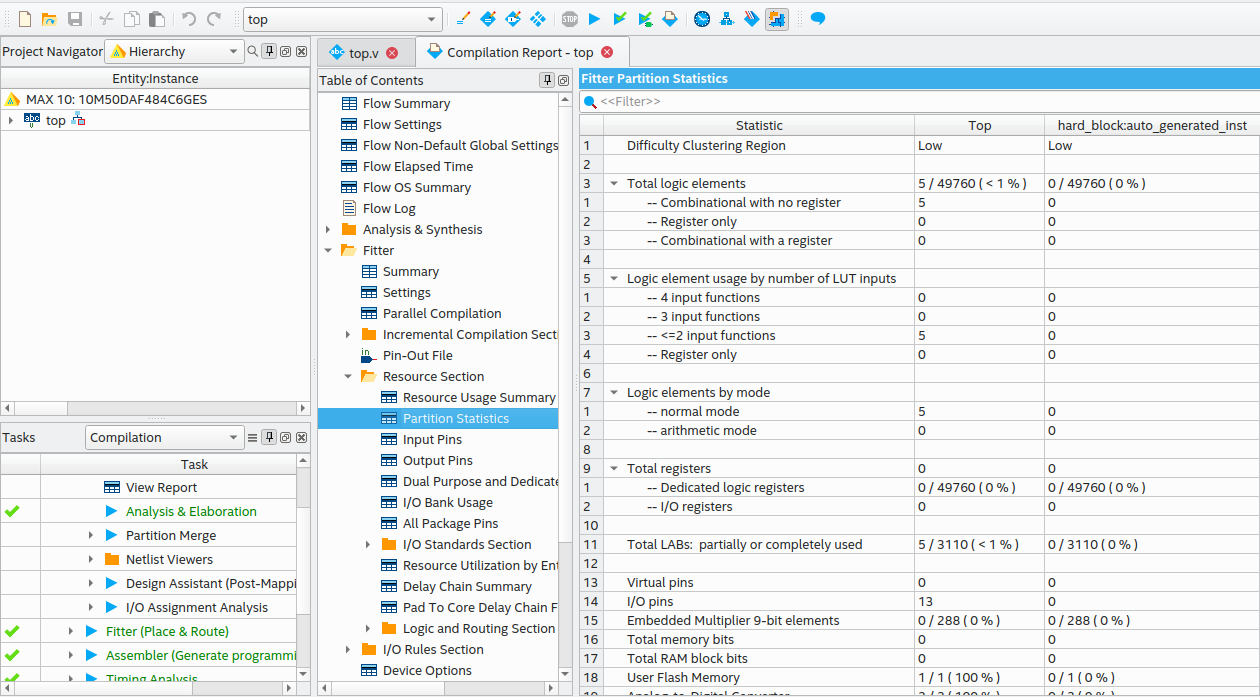
\includegraphics[width=\linewidth]{spacereport.png}
    \caption{Partition Statistics Report}
    \label{fig:partstats}
\end{figure}

\subsection{Interpreting Partition Statistics}
This report is full of useful information, and you are encouraged to read it on your own. Here we will cover just a few sections.

\textbf{Logic Element Usage:} The first 3 sections of the report provide statistics on the usage of logic elements. The first is the total logic elements, followed by look-up table (LUT) statistics, then by mode. Quartus will assign specific arithmetic logic elements when it can. We will see that in future labs.

Every FPGA has a finite number of logic elements made up of a collection of NAND or XNOR gates. You have discussed this in class. These statistics give you an idea of the space complexity of your design in terms of logic elements.

\begin{question}[Space Report]
    Capture the output of this report and include it in your final report.
\end{question}

\subsection{Timing Analysis}
Close the fitter folder and go to \directions{Logic Analyzer, Unconstrained Paths, Summary}. Your report should look something like \autoref{fig:unconstrainedpaths}. The Unconstrained Paths folder is in red, indicating a potential problem. 
\begin{figure}
    \centering
    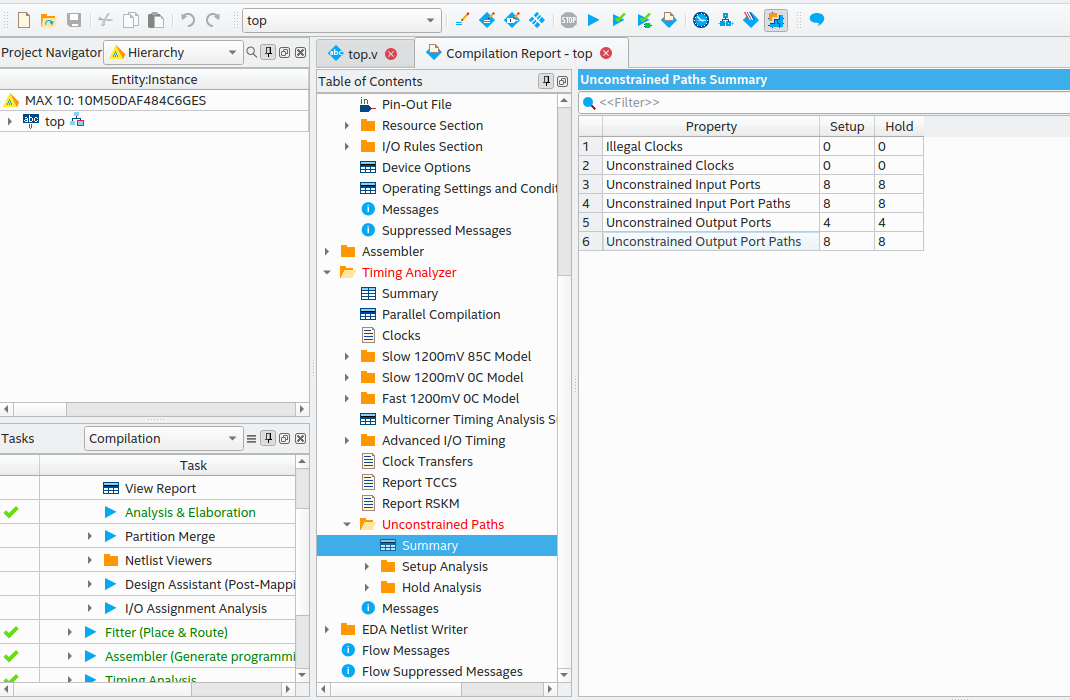
\includegraphics[width=\linewidth]{unconstrainedpaths.png}
    \caption{Unconstrained Paths Report}
    \label{fig:unconstrainedpaths}
\end{figure}

The problem in this case is that we have not provided Quartus with any timing requirements, so it cannot infer optimal routing strategies. Recall from class the discussion about timing and path delay. The worst case amount of time required to traverse a path in the circuit is called the path delay. We can and should constrain that to be within a reasonable value. This will provide the compiler with key information about how to optimize the design.

To begin, go to \directions{Tools, Timing Analyzer}. This will open a new window where we can setup our timing constraints and view additional details. When it opens for the first time it will look something like \autoref{fig:timinganalyzer}.
\subsection{Longest Path}
Before we can add constraints we need to tell the timing analyzer about our design. To do this, run the following tasks from the tasks panel (\autoref{fig:timingtasks}) in order.
\begin{enumerate}
    \item Create Timing Netlist
    \item Read SDC File
    \item Update Timing Netlist
\end{enumerate}
\begin{minipage}[t][0.5\textheight][t]{\linewidth}
\vspace{-8mm}
\begin{figure}[H]
    \centering
    \begin{tikzpicture}
        \node[anchor=center] (img1) at (0,0) {
            \begin{subfigure}{0.7\textwidth}
                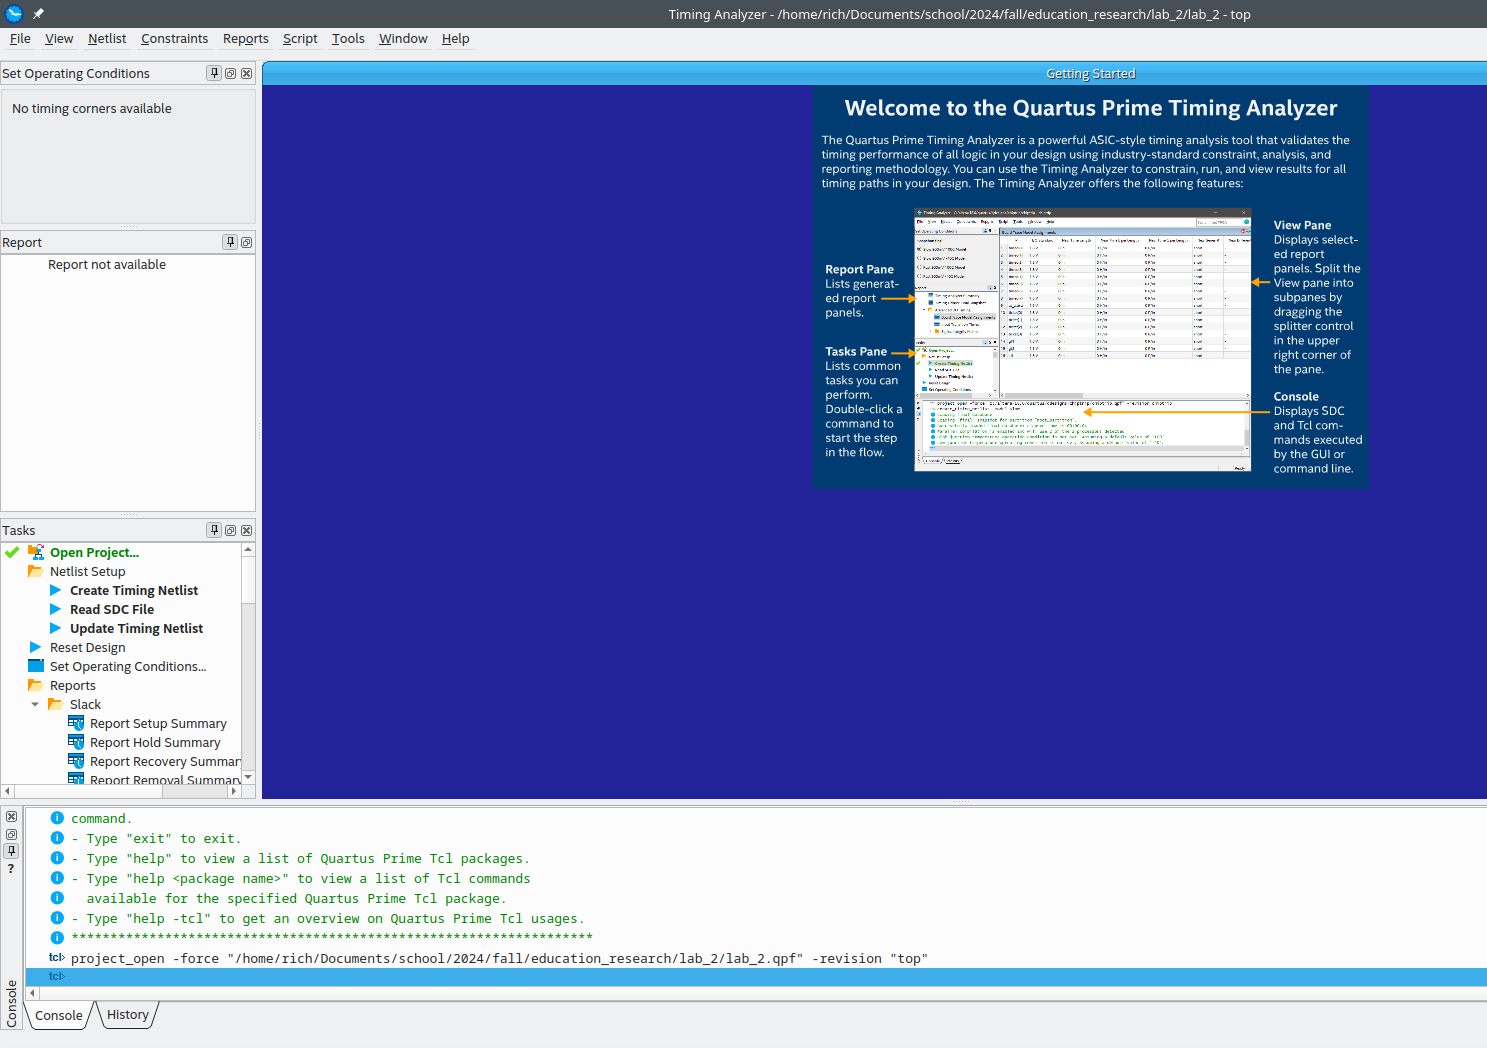
\includegraphics[width=\linewidth]{timinganalyzer.png}
                \caption{Timing Analyzer Window}
                \label{fig:timinganalyzer}
            \end{subfigure}
        };
        \hfill
        \node[anchor=center] (img2) at (8cm,0) {  % Adjust 8cm to control spacing
            \begin{subfigure}{0.2\textwidth}
                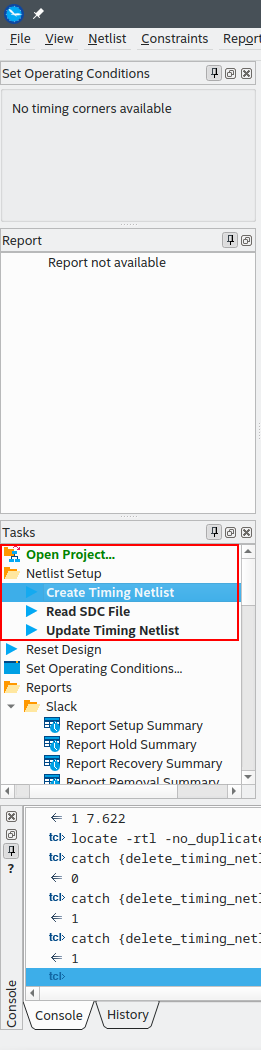
\includegraphics[width=\linewidth]{timingtasks.png}
                \caption{Timing Analyzer Tasks}
                \label{fig:timingtasks}
            \end{subfigure}
        };
        % Draw arrow from point on first image to point on second image
        \draw[<-, red, thick] ($(img1.east) - (2pt, 0pt)$) -- ($(img2.west) + (-10.5cm, 0cm)$);
        % Or for more precise positioning:
        % \draw[->, red, thick] ([xshift=2cm,yshift=1cm]img1.center) -- ([xshift=-2cm,yshift=1cm]img2.center);
    \end{tikzpicture}
    \caption{Timing Analyzer}
\end{figure}
\end{minipage}
\begin{minipage}[htbp!]{\linewidth}
\noindent
To determine a reasonable constraint, we will first check what the current maximum delay is. To do this go to \directions{Reports, Custom Reports, Report Path}. 
    \begin{minipage}[ht!]{0.5\linewidth}
    \begin{figure}[H]
    \centering
    \begin{subfigure}{\linewidth}
        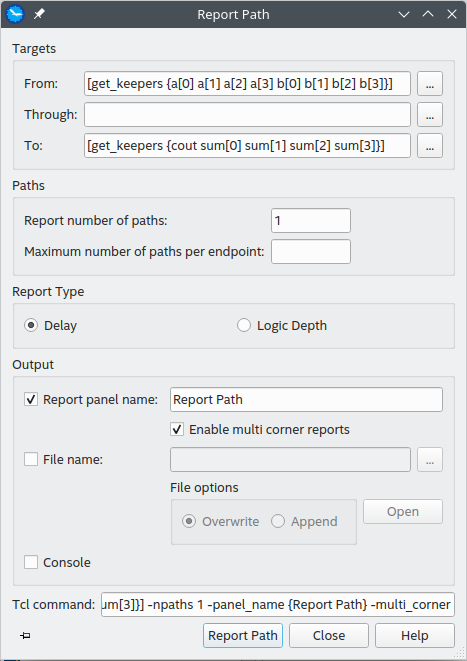
\includegraphics[width=\linewidth]{reportpath.png}
        \caption{Create Timing Report}
        \label{fig:timingreportconfig}
    \end{subfigure}
    \vspace{2mm}
    \begin{subfigure}{\linewidth}
        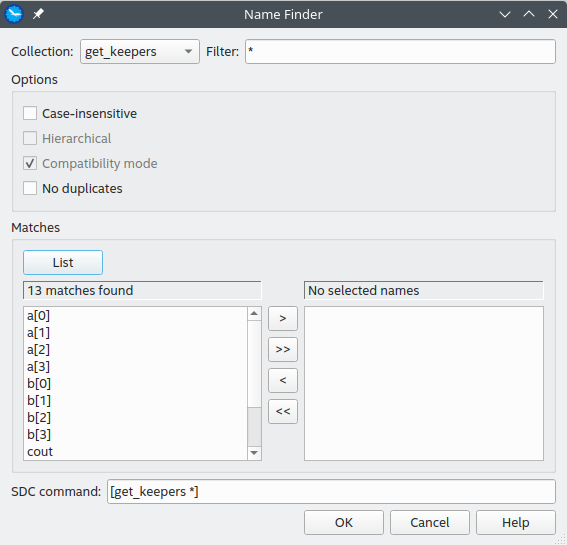
\includegraphics[width=\linewidth]{nameselection.png}
        \caption{Name Finder}
        \label{fig:namefinder}
    \end{subfigure}
    \caption{Report Setup}
    \end{figure}
    \end{minipage}
\end{minipage}%
\hspace{-0.46\textwidth}
\begin{minipage}[t]{0.45\textwidth}
\vspace{-112mm}
This will open a new dialog like that in \autoref{fig:timingreportconfig}. To populate the \keyword{From:} input, press the ellipsis button to the right of it. This will open the name finder dialog shown in \autoref{fig:namefinder}. 

Set the \keyword{Collection} option to \keyword{get\_ports}. Populate the name list in the name finder by clicking on the \keyword{List} button. Hold the \keyword{shift} button on your keyboard and select all your inputs and only your inputs. With the inputs selected, press the \keyword{$>$} button. Press \keyword{OK}. Repeat the process to populate the \keyword{To:} input, selecting \textbf{outputs only} in the name finder this time.

With \keyword{From:} and \keyword{To:} fields populated, press \keyword{Report Path}. This will generate the report in \autoref{fig:pathreport}.
\hfill\break
\begin{extra}[frametitle={Report Values}]
    The exact values in the report will differ between designs. These values depend on specific design decisions and how the compiler optimizes them.
\end{extra}
\hfill\break
\end{minipage}

\clearpage

For an overview of the longest path go to the \keyword{Path Summary} tab shown in \autoref{fig:pathreportsummary}. From here it is clear that the longest path is from second bit of the second input to the last bit of the sum. We can get a more detailed view by going to the \keyword{Data Path} tab show in \autoref{fig:pathreportdata}. This view shows every stage the signal propagates through along the path. There are several columns and rows in this report. Every row represents one stage in the longest path. Each column is defined below.
\begin{itemize}
    \item \keyword{Total}: The total time elapsed in ns
    \item \keyword{Incr}: The amount each stage contributes to the total in ns
    \item \keyword{RF}: Indicates the rise and fall charactaristics of the input and outputs of the stage. Value consist of 2 letters: \keyword{R} for rise \keyword{F} for fall. The first letter indicates the state of the signal at the input and the second letter indicates the same at the output.
    \item \keyword{Type}: Whether this delay is caused by a cell, \keyword{CELL}, or a connection between cells, \keyword{IC}.
    \item \keyword{Location}: The location of this element in the FPGA logic array.
    \item \keyword{Element}: The design element responsible for the delay.
\end{itemize}

Press the \keyword{Incr} header in the table to sort by the individual step lengths. Find the largest contributor to the overall time. In the \keyword{Element} column, right-click on the element and go to \directions{Locate Node, Locate in Technology Map Viewer}. This will open the window shown in \autoref{fig:techmap}. From here, you can see the exact hierarchy of the modules that make up the path.


\begin{figure}
    \begin{tikzpicture}
        \node (fig1) {
            {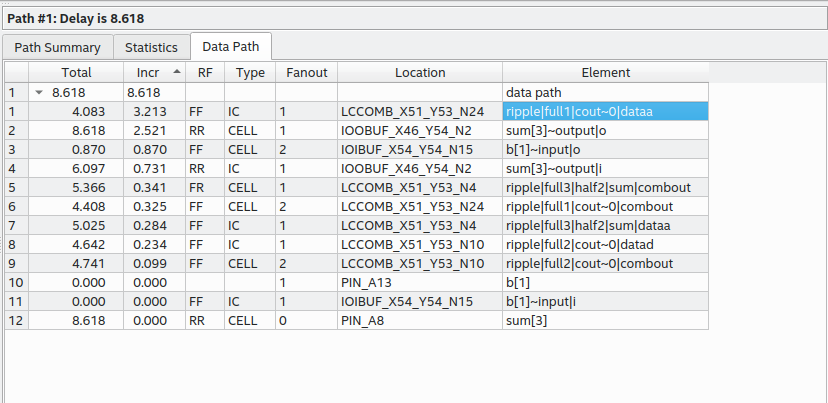
\includegraphics[width=\linewidth]{pathreport.png}}
        };
        
        % Create a box with shadow for the image
        \node[blur shadow={shadow xshift=-3pt, shadow yshift=-3pt, 
              shadow blur steps=8}] (shadowimg) at ([xshift=5cm,yshift=-3cm]fig1.center) 
            {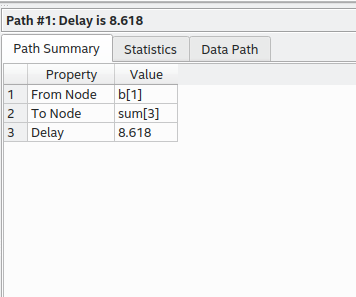
\includegraphics[width=0.5\linewidth]{pathsummaryreport.png}};
            
        % Place the caption below the shadowed image
        \node[below=1mm of shadowimg] (captiona) {
            \subcaptionbox{{}\label{fig:pathreportsummary}}
            {}
        };

               % Place the caption below the shadowed image
        \node (captionb) at ([xshift=-3cm]fig1.south) {
            \subcaptionbox{{}\label{fig:pathreportdata}}
            {}
        };
        
    \end{tikzpicture}
    \caption{Path Report: (a) Data Path (b) Path Summary}
    \label{fig:pathreport}
\end{figure}

\begin{figure}
    \centering
    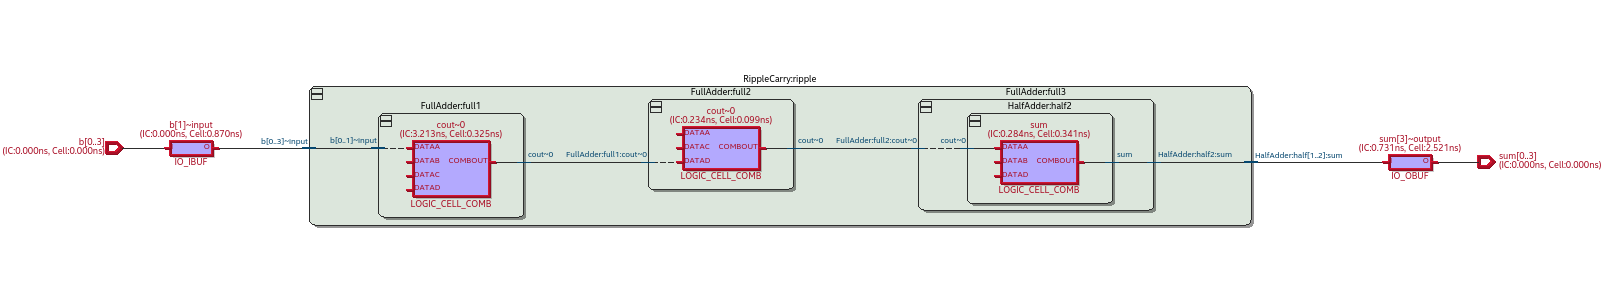
\includegraphics[width=\linewidth]{techmap.png}
    \caption{Technology Map View}
    \label{fig:techmap}
\end{figure}
\hfill\break
\begin{question}[Longest Path]
    Capture the Longest path and the time it takes in ns. Include this information in your final report. If you were to include additional bits in the adder, how would you expect the time to scale? What do you think could be done to improve this?
\end{question}
\clearpage
\subsection{Timing Constraints}
With a better idea of the unconstrained timing, we can add timing constraints. To do this, go to: \directions{Constraints, Set Maximum Delay}. This will open a new dialog with the same \keyword{from} and \keyword{to} fields we saw in the previous report. Fill them out in the same way, using the inputs for the \keyword{from} field and the outputs for the \keyword{to} field. For \keyword{Delay Value}, use a value slightly smaller than your current max time. For example, if your values were those shown in this lab packet, 7ns would be a reasonable value to choose. Press \keyword{Run} to apply the results. Finally, go to \directions{Constraints, Write SDC File}. Save the file as \keyword{top.sdc}.
\hfill\break
\begin{question}[Improvement]
\begin{enumerate}
    \item Close the timing analyzer, recompile the design, and repeat the steps in this section starting from Subsection \textbf{\ref{ss:spaceanalysis} - Space Analysis}. Was there an improvement in the longest path? What about in the space used? Why do you think that is?
    \item Update the timing constraint to a value of \keyword{5ns}. Save the SDC file and recompile. Check the path report again. Was the design able to meet the constraint? Why do you think that is the case?
\end{enumerate}
    
\end{question}

\subsection{Programming the FPGA}
To put your design on the FPGA go to: \directions{Tools, Programmer}. This will open up the programmer shown in \autoref{fig:programmer}. Press the \keyword{Hardware Setup} button to open the hardware setup dialog shown in \autoref{fig:hardwaresetup}. Select your device from the \keyword{Currently Selected Hardware} dropdown. Close that window and press the \keyword{Auto Detect} button in the Programmer window. Finally, press \keyword{Start} to program the board.
\hfill\break
\begin{extra}[frametitle={No Device Found}]
    If you do not have options in the select hardware dropdown, make sure that you have installed the USB drivers correctly. Also, check the permissions for the user running Quartus. If you still have problems, contact the TA for help.
\end{extra}


\begin{figure}[htbp!]
    \centering
    \begin{subfigure}{0.45\textwidth}    
    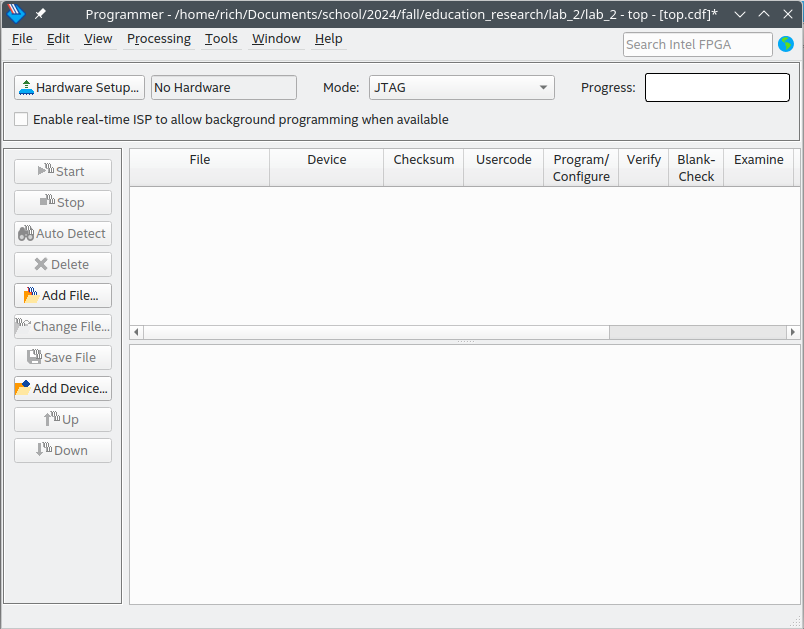
\includegraphics[width=1\linewidth]{programmer.png}
    \caption{Programmer}
    \label{fig:programmer}
    \end{subfigure}
    \hfill
    \begin{subfigure}{0.45\textwidth}
        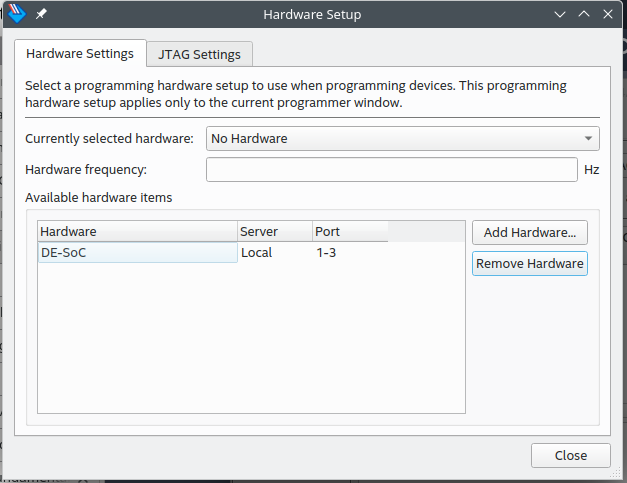
\includegraphics[width=1\linewidth]{hardwaresetup.png}
        \caption{Hardware Setup}
        \label{fig:hardwaresetup}
    \end{subfigure}
    \caption{}
\end{figure}

\hfill\break

\begin{important}[frametitle={TA Checkoff}]
    Make sure that you have demonstrated your working design to the TA before continuing.
\end{important}



\section{Carry lookahead adder}
The previous section on timing has (hopefully) made it clear that the main contributor to the delay in a ripple carry adder is the sequential carry from one node to the next. The fundamental insight behind the carry lookahead design is that we can pre-compute the value of the carryout without propagating through the stages. This is not obvious, and a thorough explanation and proof is offered in section \textbf{3.4} of the textbook.
\hfill\break
\begin{question}[Carry Lookahead Design]
\begin{enumerate}
    \item Review section \textbf{3.4} of the textbook. Design a 4-bit and an 8-bit carry lookahead adder.
    \item Write a test bench for this design, simulate it, and verify it behaves correctly. Capture the output and include it in your final report.
    \item Replace the ripple carry adder in your top level module with the carry lookahead.
    \item Recompile the design and capture the space and timing information just as done previously. Include this information in your report.
    \item Reflect on the differences in the reported values between the designs. Do you notice any trend?
\end{enumerate}
    
\end{question}


\section{Design Challenge (Extra Credit)}
Bob works at Silicon Speedsters Inc., where the CEO is obsessed with "going fast." After implementing a 2-bit carry lookahead adder that made the company millions, the CEO demanded bigger and BIGGER versions, convinced that more bits equals more profit.

Poor Bob tried explaining that carry lookahead adders grow... enthusiastically... in terms of hardware, but the CEO wouldn't listen. "Make it bigger!" he shouted, while dramatically waving his arms.

Help Bob create a graph showing how the time (delay) and space (hardware/gates) requirements grow as the bits increase from 2 to 10 bits. Maybe then the CEO will understand why they can't build that 256-bit carry lookahead adder he's dreaming about. (Bonus points if you can spot the exact moment when Bob's sanity begins to crack under the exponential growth curve.)

Note: For maximum entertainment value, please use different colored markers for the time and space plots. The CEO is also colorblind, but that's a problem for another day.
\end{document}